
% This template has been edited from the IEEE template available at:
% https://www.ieee.org/conferences/publishing/templates.html
%
% For further help, you may wish to see:#
% https://www.overleaf.com/learn/latex/tables
% https://www.overleaf.com/learn/latex/Inserting_Images
% https://www.overleaf.com/blog/532-creating-and-managing-bibliographies-with-bibtex-on-overleaf

\documentclass[conference]{IEEEtran}
%\IEEEoverridecommandlockouts
% The preceding line is only needed to identify funding in the first footnote. If that is unneeded, please comment it out.
\usepackage[a4paper, total={6in, 8in}, margin=0.75in]{geometry}
\usepackage{cite}
\usepackage{amsmath,amssymb,amsfonts}
\usepackage{algorithm} 
\usepackage{algpseudocode} 
\usepackage{graphicx}
\usepackage{textcomp}
\usepackage{xcolor}
\usepackage{color,soul}
\usepackage{float} % to allow figures across 2 columns

\def\BibTeX{{\rm B\kern-.05em{\sc i\kern-.025em b}\kern-.08em
    T\kern-.1667em\lower.7ex\hbox{E}\kern-.125em}}
\begin{document}

\title{Achieving Robot Accuracy Through Onboard Calibration, Sensors and Processing}

\author{
    \IEEEauthorblockN{xq19351}
    \and
    \IEEEauthorblockN{xl19540}
}

\maketitle

\begin{abstract}
It is normal to write the abstract last.  First, try to concisely state the problem/question/challenge under investigation.  Second, state what you found out.  The abstract should help a reader decide if they are interested in reading the whole paper.  Keep your abstract short.  Don't rely on the abstract to introduce your work.
\end{abstract}


\section{Introduction}\label{sec:intro}

% The use of robotics in industry for manufacturing and assembly processes is increasing due to improvements in software and robot manufacturing. One of the key limitations faced by robots in industry is accuracy rather than precision. This can be achieved through the use of sensors or odometry, as well as highly accurate manufacturing techniques. Without either of these features, industrial robots can be precise but not accurate requiring manual calibration when they are set up \cite{self_calibration}. This comes down to increased costs and therefore lower uptake of robotics in industry. This report aims to design a method of calibration that improves the accuracy of the Polulu 3Pi+ robot using only the onboard sensors and processors. By minimising the required human interaction, calibration can be made quicker and cheaper, hence the project aims to define an automated process on a pre-designed circuit. 


The evolution of mobile robotics is rapidly advancing, driven by significant improvements in both software and hardware technologies. 
Used for logistics, deliveries assembly lines etc. 
One of the key challenges when deploying autonomous mobile robots is accurate odometry. Robot needs to know where it is.
Mobile robots, which navigate autonomously in various environments, rely heavily on precise odometry to determine their position and movement over time. 
Odometry, a critical technique for these robots, involves the use of data from motion sensors to estimate changes in position based on wheel rotation or other locomotive mechanisms.
A major challenge for industrial robots is achieving accuracy, not just precision. 
Accuracy requires a detailed understanding of a robot's dimensions through a process called odometry. 
One of the foundational elements of robot accuracy is odometry, which requires precise knowledge of a robot's key dimensions.
Slight manufacturing tolerances can cause slight changes in the dimensions of a robot, requiring manual calibration for each robot to be accurate.
This is often achieved through manual calibration, a slow process that is prone to user error.
Impractical for swarm robotics. too many robots to manually calibrate.
Without such improvements, robots may require manual calibration at setup, increasing costs and slowing broader adoption. 
This report proposes an automatic calibration method that improves the accuracy of the Polulu 3Pi+ robot using its onboard sensors and processors, aiming to reduce the need for time-consuming manual adjustments.
By minimising the required human interaction, calibration can be made quicker and cheaper.
calibration at a low cost

\hl{define systematic vs non-systematic errors}
Systematic errors are the result of onboard errors in robot dimensions, sensors or actuators. Non-systematic errors are random errors that are caused by variation in the robot's environment and cannot be predicted or controlled.

'By accurately calibrating the odometry system, systematic errors can be minimized, resulting in more reliable estimates of the robot’s position and orientation.' \cite{odometry}

The 3Pi+ is a robot designed for learning and as such is manufactured cost-effectively meaning that component tolerances and sizing can vary. As a result, well-programmed robots will produce precise but potentially inaccurate results when tested for tasks that require accurately angled or distanced movements. 

\begin{figure}[h!]
    \centering
    \includegraphics[width = 0.45\textwidth]{img/robot_dimensions.png}
    \caption{}
    \label{fig:}
\end{figure}

Among the 3Pi+'s extensive range of sensors, the robot contains wheel encoders and infrared-radiation (IR) sensors 

\hl{datasheet} 

The wheel encoders are used to as part of the odometry and kinematics systems within the onboard code to allow the robot to determine accurate global positioning. This is similar to the majority of robotic systems and therefore provides a connection between this report and real-world industrial robotics. The encoders use \hl{explain encoders briefly}. The IR sensors are generally used to detect a line by detecting the difference in the reflected IR from a surface. For this use case the line sensor thresholds must be set for the environmental conditions in which the robot will be operating, with a clear limitation being that an inaccurate line sensor can produce inaccurate calibration results. 




\hl{add more references about calibration and reasoning as well as manufacturing defects in polulu}


\subsection{Hypothesis Statement}

through completing tests with sensor feedback, a robot can understand its own dimensions

by driving around a calibration circuit, using the 3Pi+'s built-in infrared sensors, the robot can calculate its own critical dimensions, reducing errors in the kinematics


\begin{quote}
    \emph{
     we hypothesise that the robot can measure its major dimensions and improvement its onboad kinematics through automated calibration using a known calibration circuit and the onboard sensors and processor. 
     We predict that the dimensions of the robot are a key factor in the accuracy of the robot and that this calibration process will result in a significant improvement in accuracy when compared to using the datasheet for robot dimensions.
     We also hypothesise that an automated calibration process is more timely and therefore applicable for a swarm
    }
\end{quote}

\hl{one hypothesis that its better overall and faster}
\hl{another hypothesis is that the manual calibration is better but more timely and not feasible for a swarm.}

This hypothesis will be tested by two accuracy tests on the robot. 
The hypothesis will be enacted by creating a calibration code that works on a predefined test circuit, and then the robot is tested using both the UMBmark test and a straight line distance. 
The first test will confirm the heading angle (theta) error and the second will confirm a distance error. 
If both of these tests indicate a better performance after calibration then the hypothesis will be accepted.

By minimising the human interaction required this process can be made quicker and cheaper, hence the use of automated measurements on a pre-designed circuit.

\section{Implementation}\label{sec:implementation}




\begin{algorithm}

\caption{Calibration Method} 
    \label{algo:calibration}
\textbf{Input:} Line sensor readings left to right:  linesensor[0,1,2,3,4], known length \textbf{and} angle \\
 \textbf{Output:} Array of dimensions, $R_0,R_1,L$\\

    \begin{algorithmic}
        \State State = 1
        
        \State \textbf{Update state:}
        \If{State = 1
        \textbf{and} linesensor[0] \textbf{and} linesensor[4]}
            \State State = 2
        \ElsIf{State = 2 \textbf{and} \textbf{not} linesensor[0] \textbf{and} \textbf{not} linesensor[4]}
            \State Update encoder counts
            \State State = 3
        \ElsIf{State = 3 \textbf{and} linesensor[0] \textbf{and} linesensor[4]}
            \State Calculate $R_0, R_1$ \textbf{or} $L$ 
            \State State = 4
        \EndIf\\
        
        \State \textbf{State Actions:}
        \If{State = 1 \textbf{or} State = 2 \textbf{or} State = 3}
            \State Follow line
        \ElsIf{State = 4}
            \State Stop motors
            \State Print $R_0,R_1,L$
        \EndIf
    \end{algorithmic}
\end{algorithm}


\begin{equation}
\label{eq:linear}
    R_i = \frac{C \times d}{2 \times \pi \times \Delta e_i}
\end{equation}


\begin{equation}
L = \left|\frac{\pi \times (\Delta e_0 \times R_0 - \Delta e_1 \times R_1)}{\alpha \times C}\right|
\end{equation}

Where $R_i$ are the radii of the wheels, $C$ is the number of encoder counts per revolution, $d,\alpha$ are the circuit parameters: straight line distance and turn angle and $e_i$ are encoder counts for each wheel.




\section{Experiment Methodology}\label{sec:experiment_method}


\begin{itemize}
    \item Run baseline accuracy tests for a number of robots. (linear distance and square error)
    \item Run the calibration procedure to identify new dimensions for the robot.
    \item Test the calibrated robots on the same set of accuracy tests.
    \item Identify if there is an improvement.

\end{itemize}

\subsection{Overview of Method}


There will be two experiments used to measure the outcomes of the hypothesis. The first will measure the heading angle accuracy through a test similar to the UMBmark \hl{(https://websites.umich.edu/~johannb/Papers/paper60.pdf)}. The robot will be programmed to complete 2 laps of 500mm by 500mm metre square clockwise and then anticlockwise. The resulting errors from the origin after the circuits will be used to calculate an overall heading error. The second test will measure the distance accuracy of the robot, it will be programmed to complete a straight line of length 500mm and the error recorded.

These experiments will be completed prior to the application of the calibration algorithm (described later) to establish a baseline set of results. With a baseline set of results, the calibration algorithm will be applied:

\hl{[explanation of rising edge to rising edge measurement of distance with figure]}

A printed circuit will be used for calibration, this printed circuit will be a black line printed on white paper and will form a straight line followed by an angle section. The straight line will have markers to identify a certain distance, e.g. two markers spaced 200mm apart, perpendicular to the straight line.

The robot will be tasked to complete the calibration circuit using a calibration script. After completing the straight line section, the robot will calculate the difference between the perceived kinematic reading and the known distance and will use this to calculate and store new values for the radii of the wheels. After completing the angle section of the course, the robot will calculate the difference between the perceived kinematic reading of heading and the known heading at the end of the circuit. It will use this difference to calculate and store a new value for the length of the wheelbase.

Upon completion, the robot will enter a state in which it repeatedly prints these new values to the serial monitor. These values will then be updated manually in the kinematics of that robot.

Finally the robot will be tasked to repeat the original two experiments, and the new readings of heading error and distance error will be recorded.




\subsection{Discussion of Variables}


\begin{itemize}
    \item \textbf{Controlled Variables}: For each test (baseline or otherwise) the \emph{test distances} for the straight line and the square and the number of square repeats will be kept constant. Furthermore, \emph{lighting} will be controlled ensuring that the same lighting set-up is used for all tests and calibration runs. For all robot tasks new batteries will be used.
    \hl{same PID tuning, gearbox}.
    \item \textbf{Independent Variable}: As the experiment relies on autonomous measurement by the robot, the only changing variable will be the robot, and as a result the robot dimensions - $R_0, R_1, L$. We aim to observe a measurable difference in these parameters between robots and use this to explain any improvements in system accuracy or precision after calibration. It is understood that other robot features may also vary between the robots: \hl{the gearbox backlash etc} however this report predicts that such difference result in a lower magnitude error in accuracy and as such will not impact the analysis of results.
    \item \textbf{Dependent Variable(s)}: this experiment aims to measure the accuracy and precision of the robots before and after calibration. The metrics used for quantifying the accuracy are the absolute linear error for linear tests, and orientation error and absolute position error on return-to-home on the UMBmark test.
\end{itemize}


\subsection{Discussion of Metric(s)}


\hl{comparison against manual calibration}

The key variables that we will be looking to change through calibration are:
\begin{enumerate}
    \item Radii of the wheels
    \item The width of the wheelbase
\end{enumerate}

We will be measuring the outcomes on the following variables:
\begin{enumerate}
    \item \hl{or percentage} Linear error
    \item Orientation error
    \item Absolute position error
\end{enumerate}

\hl{t-test of results is a metric}

the absolute linear error is used as it can clearly demonstrate the error from overshoot and undershoot, and needs only to be compared against performance over the same distance. The percentage error can be extracted but does not aid in improving the visibility of results. This metric will only be relevant to the measurement of the wheel radii $R_0, R_1$ as it is conducted on a straight line section and the distance is unrelated to the wheelbase $L$ as seen in equation \ref{eq:linear}.

To assess the orientation error, the UMBmark bi-directional square test is used as it allows orientation errors to accumulate and the systematic error to be found. The orientation error is measured as the degrees difference from perpendicular on return of the robot to the origin. This metric measures the accuracy of the wheelbase estimate in the kinematics of the robot as the wheelbase width is the only variable with direct impact on systematic orientation error.

Finally, the absolute position error encompasses an overall odometry systematic error found for each robot. This provides an overall measure of robot accuracy and precision. The spread of error corresponds to the overall precision and the mean values correspond to the overall accuracy. This metric and both of these observations provide a clear comparison point between robot performance pre and post calibration.



\section{Results}\label{sec:results}

\begin{figure}[]
    \centering
    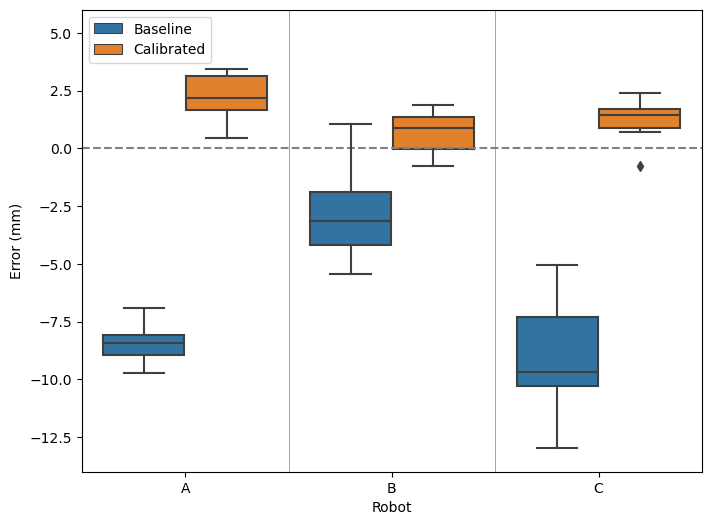
\includegraphics[width=.45\textwidth]{img/linear_pre_post.png}
    \caption{Linear error over 500mm before and after calibration}
    \label{fig:linear}
\end{figure}

\begin{figure}[]
    \centering
    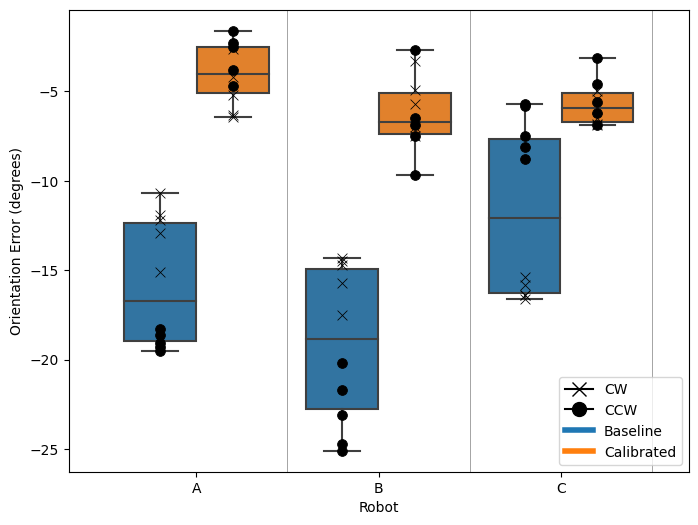
\includegraphics[width=.45\textwidth]{img/orientation_error.png}
    \caption{Orientation error before and after calibration}
    \label{fig:orientation}
\end{figure}


\begin{figure*}[]
    \centering
    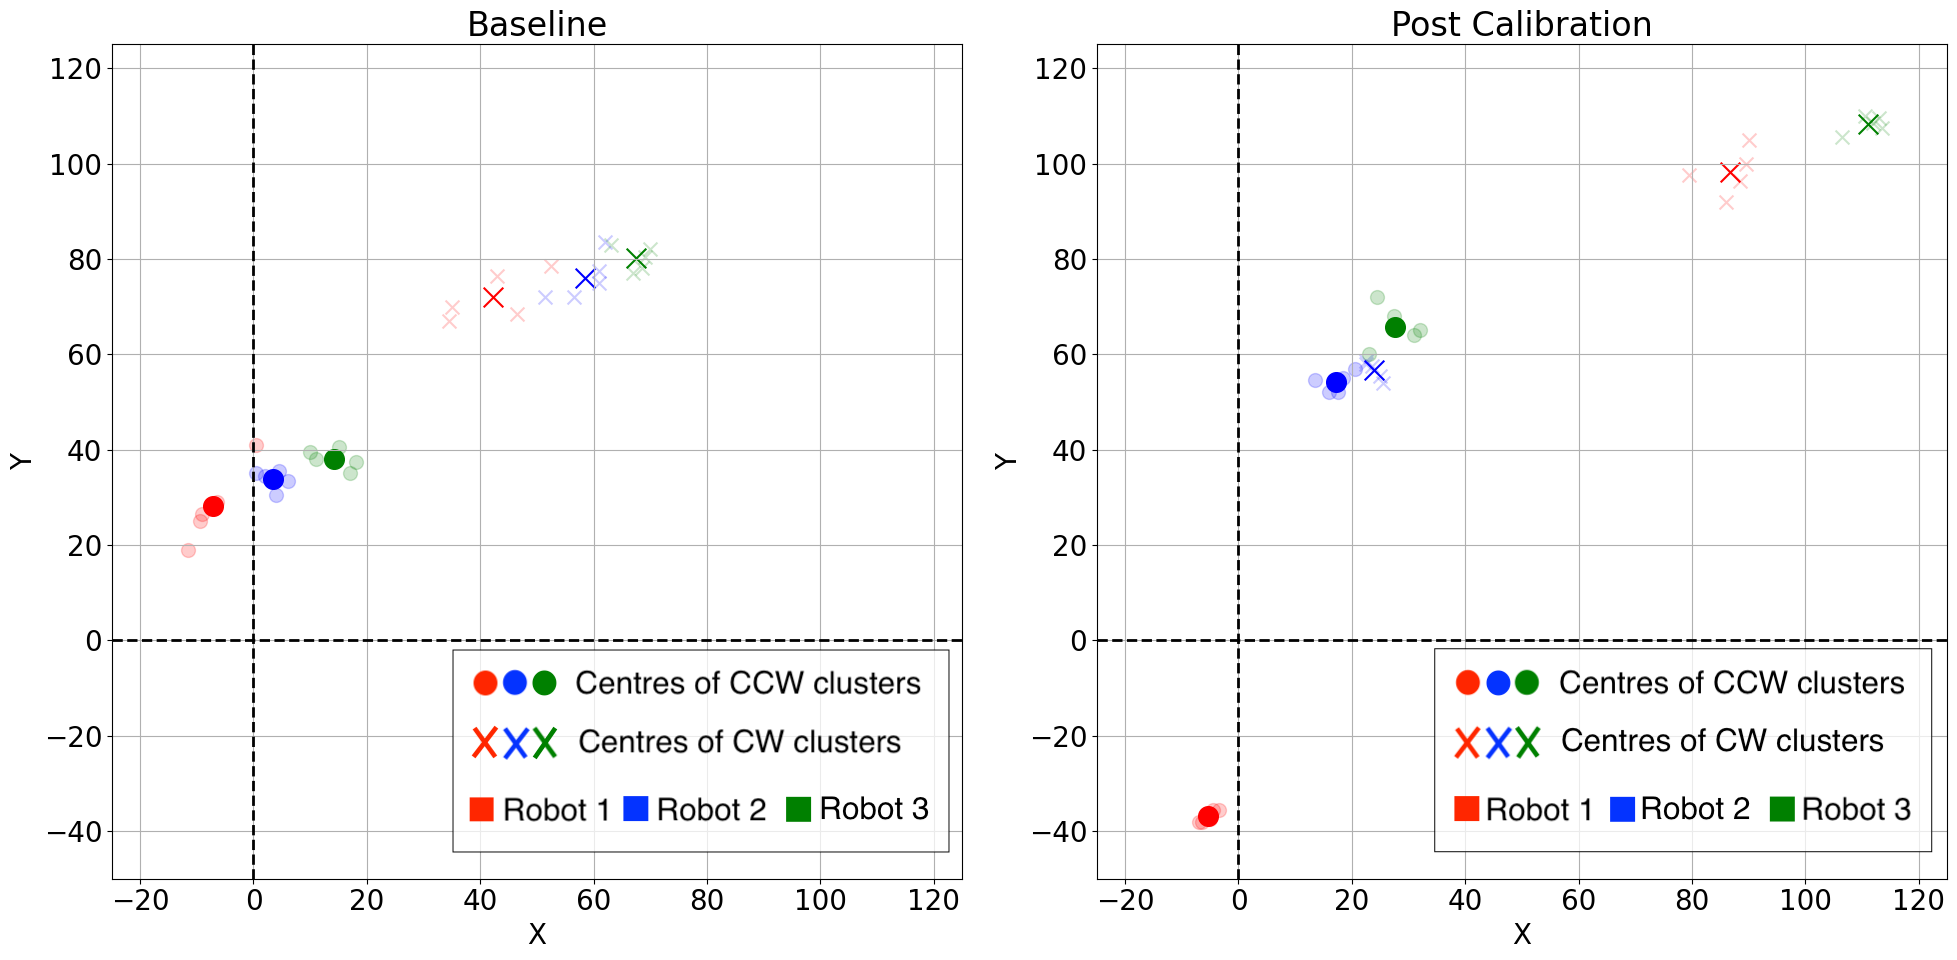
\includegraphics[width=.8\textwidth]{img/xy_pre_post.png}
    \caption{Return to home position relative to the origin for all three robots in the clockwise and anticlockwise direction. The darker marks show the mean location for each cluster.}
    \label{fig:xy_scatter}
\end{figure*}

\begin{figure}
    \centering
    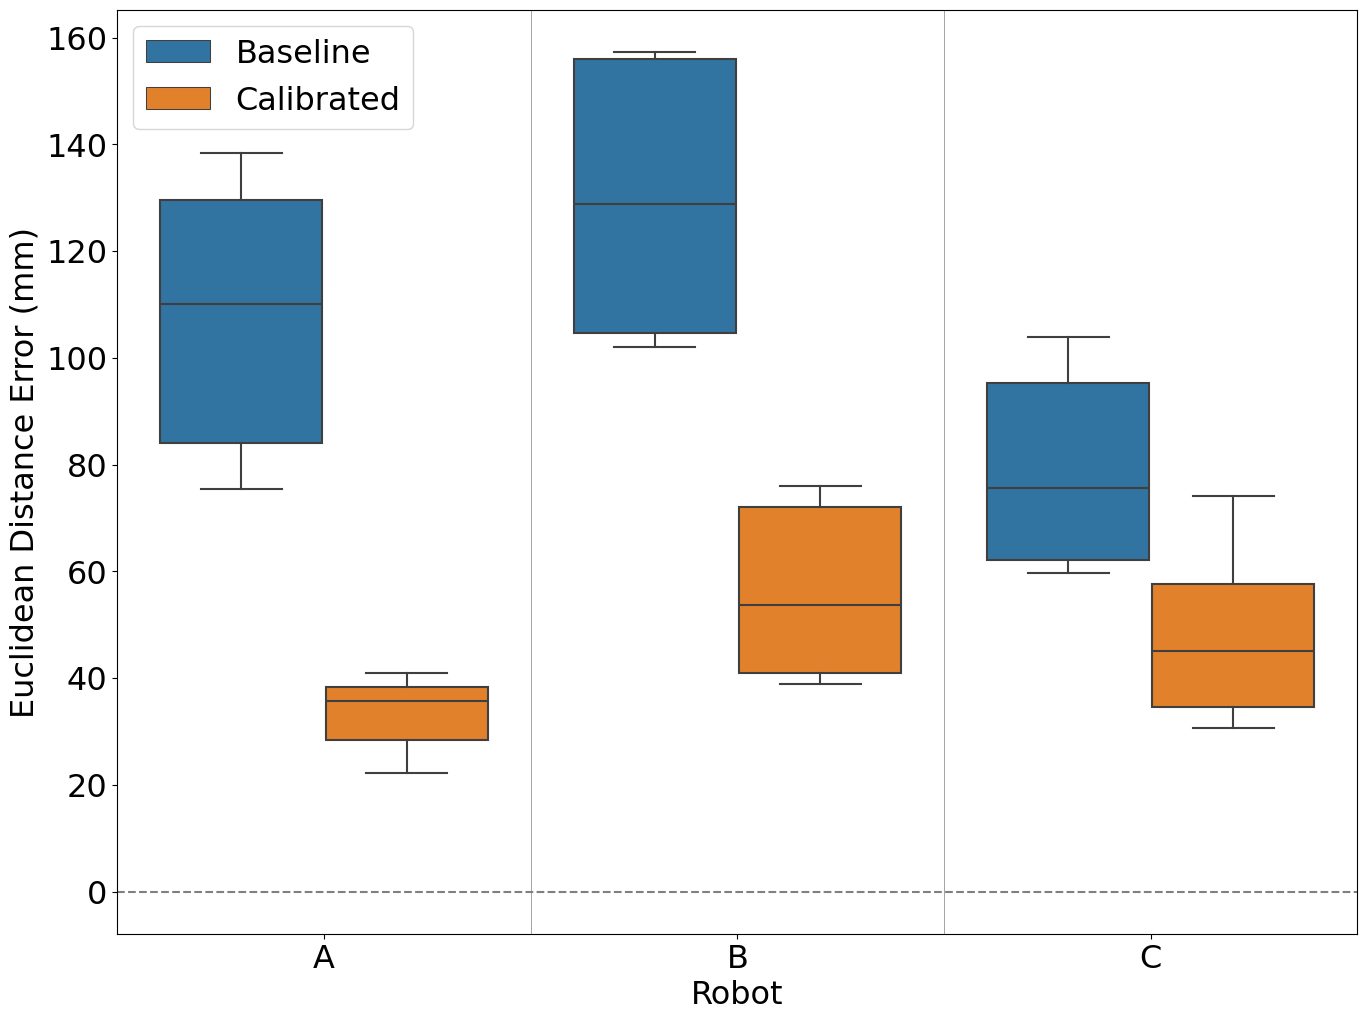
\includegraphics[width = 0.45\textwidth]{img/xy_error_boxplot.png}
    \caption{The euclidean distance error in return to home position before and after calibration.}
    \label{fig:xy_box}
\end{figure}

\hl{fig1 discuss absolute error and percentage improvements in each of the test groups }


\textbf{Assessing the results for statistical significance:} a paired t-Test has been used to assess the significance of the results for each robot. A paired t-Test is selected as the variance of results before and after calibration is not assumed to be equal as this could be impacted by the calibration. For all tests, the null hypothesis assumes that there is no difference in the means of the results before and after calibration, while the alternative hypothesis of this one-tail test states that the mean error has reduced for each robot. The tests are performed at a 5\% significance level.

For all robots, the return to home error paired  t-test found the difference between means to be
significant ($n = 10$, one-tail $p < 0.05$). The average effect size is 2.42 which means that
the post-calibration errors are more than two standard deviations lower than the pre-calibration error scores. This is considered a very large effect size. Similarly, for the linear test results, the reduction in mean absolute error is found to be significant ($n = 10$, one-tail $p < 0.05$) for all robots with an average effect size of 6.7, meaning that the average error post-calibration was over six standard deviations lower than the pre-calibration linear error.



\begin{table}[]
\centering
\caption{Paired t-Test for each robot comparing the absolute return to home error pre and post calibration.}
\label{tab:xy-test}
\begin{tabular}{l|l|l|l|l}
                                         & A       & B       & C       & Average \\ \hline
$\Delta \mu$ & 73.95   & 73.81   & 30.13   &         \\ \hline
$p(T\leq t)$                        & 1.54E-6 & 2.92E-9 & 1.08E-2 &         \\ \hline
Effect Size                              & 2.88    & 2.77    & 1.62    & 2.42   
\end{tabular}
\end{table}


\begin{table}[]
\centering
\caption{Paired t-Test for each robot comparing the absolute linear error pre and post calibration.}
\label{tab:linear-test}
\begin{tabular}{l|l|l|l|l}
                                         & A        & B       & C       & Average \\ \hline
$\Delta \mu$ & 10.70    & 3.62    & 10.25   &         \\ \hline
$p(T\leq t)$                        & 2.45E-11 & 3.07E-4 & 3.59E-7 &         \\ \hline
Effect Size                              & 13.78    & 1.90    & 4.45    & 6.71   
\end{tabular}
\end{table}


\begin{table}[h]
\centering
\caption{Paired t-Test for each robot comparing the difference in error for CW and CCW tests, showing the p-value for both pre and post calibration.}
\label{tab:cw-ccw}
\begin{tabular}{l|l|l|l}
                                  & A      & B      & C      \\ \hline
Pre-calibration $p(T \leq t)$  & 0.0002 & 0.0000006 & 0.0001 \\ \hline
Post-calibration $p(T \leq t)$ & \textbf{0.051}  & 0.0001 & 0.001 
\end{tabular}
\end{table}

It is seen in figure \ref{fig:orientation} that the distribution of error appears to be grouped based on the direction (CW or CCW) in which the square is completed for the baseline results, while the calibrated results appear to show less grouping and better overall precision. To confirm this, a hypothesis test has been conducted using a one-tailed paired t-Test at a 5\% significance level. The test outputs are summarised in table \ref{tab:cw-ccw} and show the p-value for null hypothesis: \emph{that there is no significant difference between the error for CW and CCW tests.} From the test results it can be concluded that pre-calibration there exists a significant difference ($n = 5$, one-tail $p < 0.05$) between the CW and CCW results. The post-calibration results imply that there is a reduction in this grouping effect as all p-values have increased by at least one order of magnitude. Furthermore, the grouping of the results for robot A suggests that there is insufficient evidence to reject the null hypothesis ($n = 5$, one-tail $p > 0.05$) and as such the calibration process has removed the difference between the CW and CCW performance of the robot.



\section{Discussion and Conclusion}\label{sec:discussion_conclusion}

\hl{limitations}
- gearbox slip
- linesensors and lighting
- you already need a calibrated a PID,tuned to only one robot
- battery
- wheel sizes are limited
- Relies on the accuracy of the printed calibration sheet
- Limits of the kinematic model - assumes linear movements does not calculate arcs or something like that

'It assumes that wheel revolutions directly correspond to linear displacement, neglecting factors such as wheel slippage, terrain variations, and mechanical imperfections' \cite{odometry}


\hl{further work:}
automation, ensure that the external features are accounted for better? - lighting and gearbox
counts per rev




\bibliographystyle{ieeetr} 
\bibliography{biblio}


\end{document}
